% (c) 2012-2013 Claudio Carboncini - claudio.carboncini@gmail.com
% (c) 2012-2014 Dimitrios Vrettos - d.vrettos@gmail.com

\section{Esercizi}
\subsection{Esercizi dei singoli paragrafi}
\subsubsection*{\thechapter.1 - Prime definizioni}

\begin{esercizio}
\label{ese:G.1}
Completate la figura mettendo le opportune lettere ai vertici dei triangoli rettangoli assegnati e, applicando le definizioni, scrivete la formula
che permette di ricavare l'elemento incognito indicato con un punto interrogativo a partire dagli elementi noti indicati con una lettera.
\begin{center}
 % (c) 2012 Dimitrios Vrettos - d.vrettos@gmail.com

\begin{tikzpicture}[x=10mm,y=10mm, font=\small]
  \coordinate (A) at (0,0);
  \coordinate (B) at ($(A)+(0:-2)$);
  \coordinate (C) at ($(A)+(90:3)$);

  \draw (C)--(A)--(B)--(C);

  \tkzMarkAngle[fill=LimeGreen, draw=black, size=.3](B,C,A)
  \tkzLabelAngle[pos=.6, font=\scriptsize](B,C,A){$\alpha$}
  \tkzLabelSegment[midway, right](A,C){$c$}
  \tkzLabelSegment[midway](B,C){?}

  \begin{scope}[xshift=10mm, yshift=-20mm]
    \coordinate (A) at (0,0);
    \coordinate (B) at ($(A)+(0:-2)$);
    \coordinate (C) at ($(A)+(90:3)$);

    \draw (C)--(A)--(B)--(C);

    \tkzMarkAngle[fill=LimeGreen, draw=black, size=.3](A,B,C)
    \tkzLabelAngle[pos=.6, font=\scriptsize](A,B,C){$\alpha$}
    \tkzLabelSegment[midway, right](A,C){?}
    \tkzLabelSegment[midway](B,C){$c$}
  \end{scope}

  \begin{scope}[xshift=15mm, yshift=12mm]
    \coordinate (A) at (0,0);
    \coordinate (B) at ($(A)+(0:4)$);
    \coordinate (C) at ($(A)+(60:2)$);

    \draw (C)--(A)--(B)--(C);

    \tkzMarkAngle[fill=LimeGreen, draw=black,size=.4](C,B,A)
    \tkzLabelAngle[pos=.6, font=\scriptsize](C,B,A){$\alpha$}
    \tkzLabelSegment[midway](B,C){?}
    \tkzLabelSegment[midway, below](B,A){$b$}
  \end{scope}

  \begin{scope}[xshift=15mm, yshift=-15mm]
    \coordinate (A) at (0,0);
    \coordinate (B) at ($(A)+(0:4)$);
    \coordinate (C) at ($(A)+(60:2)$);

    \draw (C)--(A)--(B)--(C);

    \tkzMarkAngle[fill=LimeGreen, draw=black,size=.4](B,A,C)
    \tkzLabelAngle[pos=.6, font=\scriptsize](B,A,C){$\alpha$}
    \tkzLabelSegment[midway](B,C){?}
    \tkzLabelSegment[midway](C,A){$c$}
  \end{scope}

  \begin{scope}[xshift=70mm, yshift=8mm, rotate=40]
    \coordinate (A) at (0,0);
    \coordinate (B) at ($(A)+(0:2)$);
    \coordinate (C) at ($(A)+(90:3)$);

    \draw (C)--(A)--(B)--(C);

    \tkzMarkAngle[fill=LimeGreen, draw=black, size=.4](A,C,B)
    \tkzLabelAngle[pos=.6, font=\scriptsize](A,C,B){$\alpha$}
    \tkzLabelSegment[midway, left](A,C){$c$}
    \tkzLabelSegment[midway,above](B,C){?}
  \end{scope}

  \begin{scope}[xshift=60mm, yshift=-20mm]
    \coordinate (A) at (0,0);
    \coordinate (B) at ($(A)+(0:2)$);
    \coordinate (C) at ($(A)+(90:3)$);

    \draw (C)--(A)--(B)--(C);

    \tkzMarkAngle[fill=LimeGreen, draw=black, size=.4](C,B,A)
    \tkzLabelAngle[pos=.6, font=\scriptsize](C,B,A){$\alpha$}
    \tkzLabelSegment[midway, left](A,C){$c$}
    \tkzLabelSegment[midway,below](B,A){?}
  \end{scope}
\end{tikzpicture}
\end{center}

\end{esercizio}

\subsubsection*{\thechapter.2 - Due identità fondamentali}

\begin{esercizio}
\label{ese:G.2}
Nel triangolo rettangolo~$ABC$ sappiamo che~$\sin(\gamma )=\frac{5}{7}$.
Determinare le altre funzioni trigonometriche dell'angolo~$\gamma$ e quelle del suo complementare.
\end{esercizio}

\subsubsection*{\thechapter.4 - Usare la calcolatrice}

\begin{esercizio}
\label{ese:G.3}
Completare la tabella inserendo nelle caselle vuote misure di angoli acuti a piacere, approssimando alla quarta cifra decimale.
\begin{center}
\begin{tabular}{cccccccccc}
\toprule
$\alpha$ & $0\grado$ & \ldots & $30\grado$ & \ldots & $45\grado$ & \ldots & $60\grado$ & \ldots & $90\grado$\\
\midrule
$\cos(\alpha)$ & & & & & & & & & \\
\bottomrule
\end{tabular}
\end{center}
\end{esercizio}

\begin{esercizio}
\label{ese:G.4}
Completare la tabella inserendo nelle caselle vuote misure di angoli acuti a piacere.
\begin{center}
\begin{tabular}{cccccccccc}
\toprule
$\alpha$ & $0\grado$ & \ldots & $30\grado$ & \ldots & $45\grado$ & \ldots & $60\grado$ & \ldots & $90\grado$\\
\midrule
$\sin(\alpha)$ & & & & &  &  &  &  &  \\
$\tan(\alpha)$ & & &  &  &  &  &  &  &  \\
\bottomrule
\end{tabular}
\end{center}

Quali osservazioni si possono fare per la funzione~$\sin({\alpha}$)?
\end{esercizio}

\begin{esercizio}
\label{ese:G.5}
Nel primo esempio avevamo trovato per le funzioni trigonometriche degli angoli acuti del triangolo rettangolo di lati~$5\unit{m}$,
$4\unit{m}$ e $3\unit{m}$, i seguenti valori:
$\sin(\beta)=\frac{b}{a}=\frac{3}{5}$, $\cos(\beta)=\frac{c}{a}=\frac{4}{5}$, $\tan(\beta)=\frac{b}{c}=\frac{3}{4}$.
Determina l'ampiezza degli angoli acuti attivando le funzioni inverse sulla tua calcolatrice.
\end{esercizio}

\subsubsection*{\thechapter.5 - Operazioni con i gradi sessagesimali}

\begin{esercizio}
\label{ese:G.6}
Esegui le seguenti operazioni con gli angoli.
\begin{multicols}{2}
\begin{enumeratea}
 \item Calcola il complementare di~$25\grado~30' 58''$;
 \item Calcola il supplementare di~$118\grado~59' 5''$;
 \item Calcola il doppio di~$45\grado~45' 45''$;
 \item Calcola la metà di~$128\grado~57' 30''$;
 \item Calcola $16\grado~29' 32''+ 95\grado~57' 31''$;
 \item Calcola $127\grado~50' 32''+ 27\grado~51' 42''$.
\end{enumeratea}
\end{multicols}
\end{esercizio}

\subsubsection*{\thechapter.6 - Risoluzione di triangoli rettangoli}

\begin{esercizio}
\label{ese:G.7}%[figura~11]
Risolvere il triangolo rettangolo in figura a partire dai dati a disposizione.
\begin{multicols}{2}
\begin{center}
 % (c) 2012 Dimitrios Vrettos - d.vrettos@gmail.com

\begin{tikzpicture}[x=9mm,y=9mm, font=\small]

  \coordinate (A) at (0,0);
  \coordinate (C) at ($(A)+(90:3)$);
  \coordinate (B) at ($(A)+(0:4)$);

  \draw (A) node[below left]{$A$}-- (C) node[above left]{$C$} -- (B)node[below right]{$B$} -- (A);

  \tkzMarkAngle[ fill=LimeGreen ,draw, size=.4](A,C,B)
  \tkzMarkAngle[ fill=LimeGreen ,draw, size=.4](C,B,A)
  \tkzMarkRightAngle[ fill=LimeGreen ,draw, size=.3](C,A,B)
  
  \begin{scope}[font=\scriptsize]
    \tkzLabelAngle[pos=.6](A,C,B){$\gamma$}
    \tkzLabelAngle[pos=.6](C,B,A){$\beta$}
    \tkzLabelAngle[pos=.6](C,A,B){$\alpha$}
  \end{scope}

  \tkzLabelSegment[midway, left](A,C){$b$}
  \tkzLabelSegment[midway, below](A,B){$c$}
  \tkzLabelSegment[midway, above](B,C){$a$}

  \begin{scope}[fill=CornflowerBlue, draw=black]
    \filldraw (0,0) circle (1pt);
    \filldraw (4,0) circle (1pt);
    \filldraw (0,3) circle (1pt);
  \end{scope}

\end{tikzpicture}
\end{center}
\begin{enumeratea}
 \item $a=30\unit{cm}$,$\quad\beta=25\grado~30'$;
 \item $a=1,25\unit{m}$,$\quad\gamma=75\grado$;
 \item $a=15\unit{cm}$,$\quad\beta=30\grado$;
 \item $a=36\unit{cm}$,$\quad\sin(\beta)=\frac{2}{3}$;
 \item $c=12\unit{m}$,$\quad\cos(\beta)=\frac{1}{4}$;
 \item $c=12\unit{m}$,$\quad\tan(\beta)=2$;
 \item $b=40\unit{cm}$,$\quad\tan(\beta)=1$;
 \item $c=12\unit{cm}$,$\quad a=20\unit{cm}$;
 \item $b=30\unit{cm}$,$\quad c=40\unit{cm}$.
\end{enumeratea}
\end{multicols}
\end{esercizio}

\begin{esercizio}
\label{ese:G.8}
Nel triangolo rettangolo~$ABC$, retto in~$A$, determina l'altezza relativa all'ipotenusa sapendo che il cateto~${AB} = 20\unit{cm}$
e l'angolo~$\beta=25\grado$.
\end{esercizio}

\begin{esercizio}
\label{ese:G.9}
Sapendo che~$\cos(\gamma)=\frac{5}{12}$ e che il cateto~$b$ misura~$20\unit{cm}$, calcola area e perimetro del triangolo rettangolo.
\end{esercizio}

\begin{esercizio}
\label{ese:G.10}
Determinare perimetro e area del triangolo rettangolo~$ABC$ retto in~$A$ sapendo che l'altezza relativa all'ipotenusa misura~$0,5\unit{cm}$
e l'angolo~$\alpha$ è di~$30\grado$.
\end{esercizio}

\paragraph{Proiezione di un segmento lungo una direzione}
\begin{esercizio}
\label{ese:G.11}
Costruite la proiezione del segmento~$AB$ sulla retta~$r$ in ciascuna delle figure seguenti e descrivete i passi effettuati.
\begin{center}
 % (c) 2012 Dimitrios Vrettos - d.vrettos@gmail.com

\begin{tikzpicture}[x=10mm,y=10mm, font=\small]
\tkzDefPoints{0/0/A,1.5/1/B, 0/1.2/C}
\tkzDrawLine[add=0 and 0,thin](A,B)
\tkzDrawLine[end=$r$,thin](A,C)
\tkzMarkAngle[fill=LimeGreen, draw=black, size=.4](B,A,C)
\tkzLabelAngle[pos=.6, font=\scriptsize](B,A,C){$\alpha$}
\begin{scope}[fill=CornflowerBlue, draw=black]
\filldraw (0,0) circle (1.5pt) node[left] {$A$};
\filldraw (1.5,1) circle (1.5pt) node[right] {$B$};
\end{scope}

\begin{scope}[xshift=35mm, yshift=10mm]
\tkzDefPoints{0/0/A,2/.6/B, -1/1.2/C}
\tkzDrawLine[add=0 and 0,thin](A,B)
\tkzDrawLine[add=1 and 0,end=$r$,thin](A,C)
\tkzMarkAngle[fill=LimeGreen, draw=black, size=.4](B,A,C)
\tkzLabelAngle[pos=.6, font=\scriptsize](B,A,C){$\beta$}
\begin{scope}[fill=CornflowerBlue, draw=black]
\filldraw (0,0) circle (1.5pt) node[left] {$A$};
\filldraw (2,.6) circle (1.5pt) node[right] {$B$};
\end{scope}
\end{scope}

\begin{scope}[xshift=65mm]
\tkzDefPoints{0/0/A,1.5/0/B, 0/1.2/C}
\tkzDrawLine[add=0 and 0,thin](A,B)
\tkzDrawLine[end=$r$,thin](A,C)
\tkzMarkAngle[fill=LimeGreen, draw=black, size=.4](B,A,C)
\tkzLabelAngle[pos=.6, font=\scriptsize](B,A,C){$\gamma$}
\begin{scope}[fill=CornflowerBlue, draw=black]
\filldraw (0,0) circle (1.5pt) node[left] {$A$};
\filldraw (1.5,0) circle (1.5pt) node[right] {$B$};
\end{scope}
\end{scope}

\end{tikzpicture}
\end{center}
\end{esercizio}

\begin{multicols}{2}
 \begin{esercizio}
\label{ese:G.12}
Il segmento~$AB$ delle figura~\ref{fig:G.8} misura~$2\unit{m}$. Determinare la misura della sua proiezione~$AH$ sulla retta~$r$ sapendo che l'angolo tra retta e
segmento è di~$72\grado$. Determinare infine perimetro e area del triangolo~$AHB$.
\end{esercizio}
\begin{esercizio}
\label{ese:G.13}
Della figura~\ref{fig:G.9} sappiamo che:~${AB}=2\unit{m}$, ${DC}=2,52\unit{m}$ e ${AC}=3,76\unit{m}$.
Indicate con~$H$ e~$K$ rispettivamente le proiezioni di~$B$ e~$D$ sulla retta~$r$, determinate l'area del poligono~$ACDB$.
\end{esercizio}
\end{multicols}

\begin{figure}[t]
 \begin{minipage}[t]{.25\textwidth}
 \centering
 % (c) 2012 Dimitrios Vrettos - d.vrettos@gmail.com

\begin{tikzpicture}[x=9mm,y=9mm, font=\small]
\tkzDefPoint(0,0){A}
\tkzDefShiftPoint[A](36:2){B}
\tkzDefShiftPoint[A](0:2){C}
\tkzDefShiftPoint[A](0:1.62){H}
\tkzDrawLine[add=0 and 0, thin](A,B)
\tkzDrawLine[add=0 and 0, thin, dashed](H,B)
\tkzDrawLine[thin, end=$r$](A,C)
\tkzLabelPoints[below](A,H)
\tkzLabelPoints[above](B)
\tkzDrawPoints[	color=CornflowerBlue](A,B, H)
\end{tikzpicture}
 \caption{Es. G.12.}\label{fig:G.8}
 \end{minipage}
 \begin{minipage}[t]{.45\textwidth}
 \centering
 % (c) 2012 Dimitrios Vrettos - d.vrettos@gmail.com

\begin{tikzpicture}[x=9mm,y=9mm, font=\small]
\tkzDefPoint(0,0){A}
\tkzDefShiftPoint[A](45:2){B}
\tkzDefShiftPoint[A](0:4){R}

\tkzDefPoint(3.76,0){C}
\tkzDefShiftPoint[C](120:2.52){D}

\tkzDrawLine[add=0 and 0, thin](A,B)
\tkzDrawLine[add=0 and 0, thin](C,D)
\tkzDrawLine[thin, end=$r$](A,R)

\tkzLabelPoints[below](A,C)
\tkzLabelPoints[above](B,D)
\tkzDrawPoints[color=CornflowerBlue](A,B,C,D)

\tkzMarkAngle[fill=LimeGreen, draw=black, size=.4](R,A,B)
\tkzMarkAngle[fill=LimeGreen, draw=black, size=.4](R,C,D)
\begin{scope}[font=\scriptsize]
\tkzLabelAngle[pos=1, below](R,A,B){$\alpha=45^{\circ}$}
\tkzLabelAngle[pos=.9, below](R,C,D){$\beta=120^{\circ}$}
\end{scope}
\end{tikzpicture}
 \caption{Es. G.13.}\label{fig:G.9}
 \end{minipage}
 \begin{minipage}[t]{.25\textwidth}
 \centering
 % (c) 2012 Dimitrios Vrettos - d.vrettos@gmail.com

\begin{tikzpicture}[x=9mm,y=9mm, font=\small]
\tkzDefPoint(0,0){A}
\tkzDefShiftPoint[A](45:2){B}
\tkzDefShiftPoint[A](0:1.6){R}

\tkzDefPoint(1.44,0){H}

\tkzDrawLine[add=0 and 0, thin](A,B)
\tkzDrawLine[add=0 and 0, thin,dashed](H,B)
\tkzDrawLine[thin, end=$r$](A,R)

\tkzLabelPoints[below](A,H)
\tkzLabelPoints[above](B)
\tkzDrawPoints[color=CornflowerBlue](A,B,H)

\tkzMarkAngle[fill=LimeGreen, draw=black, size=.4](R,A,B)

\begin{scope}[font=\scriptsize]
\tkzLabelAngle[pos=.6](R,A,B){$\alpha$}

\end{scope}
\end{tikzpicture}
 \caption{Es. G.14.}\label{fig:G.10}
 \end{minipage}
\end{figure}

\begin{multicols}{2}
\begin{esercizio}
\label{ese:G.14}
La proiezione~$AH$ è di~$2$ metri (figura~\ref{fig:G.10}). Determinate la misura del segmento ``proiettante'' $AB$ nei seguenti casi:~$\alpha=28\grado$;
$\alpha=45\grado$; $\alpha=60\grado$; $\alpha=88\grado$ (con l'approssimazione alla quarta cifra decimale).
\end{esercizio}

\begin{esercizio}
\label{ese:G.15}
In un triangolo rettangolo conoscendo il coseno dell'angolo acuto~$\alpha$ vale $0,3$; calcola~$sin(\alpha)$ e~$tan(\alpha)$.
Calcola, inoltre, il valore dell'angolo acuto~$\alpha$ in gradi e decimali di grado.
\end{esercizio}

\begin{esercizio}
\label{ese:G.16}
In un triangolo rettangolo di angolo acuto~$x$, calcola~$\cos(x)$, $\tan(x)$ e~$x$ sapendo che~$\sin(x)=0,2$.
\end{esercizio}

\begin{esercizio}
\label{ese:G.17}
In un triangolo rettangolo di angolo acuto~$x$, calcola~$\sin(x)$, $\cos(x)$ e~$x$ sapendo che~$\tan(x)=1,5$.
\end{esercizio}

\begin{esercizio}
\label{ese:G.18}
In un triangolo rettangolo conoscendo il coseno dell'angolo acuto~$\alpha$, $\cos(\alpha)=0,7$ calcola~$\sin(\alpha)$ e~$\tan(\alpha)$.
Calcola, inoltre, il valore dell'angolo acuto~$\alpha$ in gradi e decimali di grado.
\end{esercizio}

\begin{esercizio}
\label{ese:G.19}
Trova area e perimetro del triangolo rettangolo~$ABC$ retto in~$A$ sapendo che~$AB=50\unit{cm}$.
\end{esercizio}

\begin{esercizio}
\label{ese:G.20}
Risolvi il triangolo rettangolo che ha un cateto di~$25\unit{cm}$ e il seno dell'angolo ad esso adiacente pari a~$0,28$.
\end{esercizio}

\begin{esercizio}
\label{ese:G.21}
In un triangolo rettangolo conoscendo il coseno dell'angolo acuto~$\alpha$, $\cos(\alpha)= 0,2$, calcola~$\sin(\alpha)$ e
$\tan(\alpha)$. Calcola, inoltre, la misura dei restanti lati sapendo che il cateto opposto ad~$\alpha$ misura~$66\unit{cm}$.
\end{esercizio}
\end{multicols}

\subsubsection*{\thechapter.7 - Risoluzione di un triangolo qualsiasi con triangoli rettangoli}

\begin{esercizio}
\label{ese:G.22}
Risolvi il triangolo acutangolo~$ABC$ nei seguenti casi.
\begin{multicols}{2}
\begin{enumeratea}
\item $\overline{CH}=20\unit{cm}$,~~$\alpha=45\grado$,~~$\beta=62\grado~20'$;
\item $\overline{AC}=20\unit{cm}$,~~$\alpha=60\grado$,~~$\beta=35\grado$;
\item $\overline{BH}=12\unit{cm}$,~~$\alpha=35\grado$,~~$\beta=40\grado~30'$;
\item $\overline{AH}=22,25\unit{cm}$,~~$\alpha=20\grado$,~~$\beta=65\grado$;
\item $\overline{CH}=10\unit{cm}$,~~$\alpha=42\grado$,~~$\beta=53\grado$.
\end{enumeratea}
\end{multicols}
\end{esercizio}

\begin{esercizio}
\label{ese:G.23}
In riferimento alla seguente figura risolvi il triangolo~$ABC$, conoscendo gli elementi indicati nei due casi (a e b).
\begin{center}
  % (c) 2012 Dimitrios Vrettos - d.vrettos@gmail.com

\begin{tikzpicture}[x=10mm,y=10mm, font=\small]
\tkzDefPoint(0,0){A}
\tkzDefShiftPoint[A](0:3){B}
\tkzDefShiftPoint[A](120:2){C}
\tkzDefPoint(-1,0){H}

\tkzDrawLine[add=0 and 0, thin](A,B)
\tkzDrawLine[add=0 and 0, thin](A,C)
\tkzDrawLine[add=0 and 0, thin](C,B)
\tkzDrawLine[add=0 and 0, thin,dashed](C,H)
\tkzDrawLine[add=0 and 0, thin,dashed](A,H)


\tkzLabelPoints[below](A,H,B)
\tkzLabelPoints[above](C)
\tkzDrawPoints[color=CornflowerBlue](A,B,C,H)

\tkzMarkAngle[fill=LimeGreen, draw=black, size=.4](B,A,C)
\tkzMarkAngle[fill=LimeGreen, draw=black, size=.4](A,C,B)
\tkzMarkAngle[fill=LimeGreen, draw=black, size=.5](C,B,A)
\begin{scope}[font=\scriptsize]
\tkzLabelAngle[pos=.6](B,A,C){$\alpha$}
\tkzLabelAngle[pos=.6](A,C,B){$\gamma$}
\tkzLabelAngle[pos=.8](A,B,C){$\beta$}
\end{scope}
\end{tikzpicture}
\end{center}
\begin{multicols}{2}
 \begin{enumeratea}
\item $\overline{AB}=2\unit{cm}$,~~$\overline{BC}=6\unit{cm}$,~~$\beta=30\grado$;
\item $\overline{CH}=50\unit{cm}$,~~$\overline{AB}=76\unit{cm}$,~~$\alpha=120\grado$.
\end{enumeratea}
\end{multicols}
\end{esercizio}

\begin{multicols}{2}
\begin{esercizio}
\label{ese:G.24}
Risolvere un triangolo isoscele nota la base$=4\sqrt{2}\unit{cm}$ e l'$\Area=32\unit{cm^2}$.
\end{esercizio}

\begin{esercizio}
\label{ese:G.25}
Un triangolo isoscele ha l'altezza relativa al lato più corto pari a~$120\unit{cm}$ e il seno dell'angolo alla base è uguale a~$\frac{2}{3}$.
Calcola perimetro e area del triangolo.
\end{esercizio}
\end{multicols}

\paragraph{Quadrilateri}
\begin{multicols}{2}
 \begin{esercizio}
\label{ese:G.26}
Nel trapezio isoscele~$ABCD$, la base minore $CD$ misura~$30\unit{cm}$, i lati obliqui~$20\unit{cm}$
e il seno degli angoli acuti è~$0,6$. Trova la misura del perimetro e dell'area.
\end{esercizio}

\begin{esercizio}
\label{ese:G.27}
Trova l'area di un rombo di perimetro~$120\unit{cm}$ e con gli angoli ottusi ognuno pari a~$100\grado$.
\end{esercizio}

\begin{esercizio}
\label{ese:G.28}
Trova la misura del lato e dell'altezza del rombo con diagonale maggiore di~$20\unit{cm}$ e con uno dei due angoli acuti di~$30\grado$.
\end{esercizio}

\begin{esercizio}
\label{ese:G.29}
Trova le due altezze del parallelogramma di lati~$10\unit{cm}$ e~$15\unit{cm}$ e con i due angoli acuti ognuno di~$20\grado$.
\end{esercizio}

\begin{esercizio}
\label{ese:G.30}
Trova l'area di un parallelogramma sapendo che i lati sono lunghi~$12,5\unit{cm}$ e~$7,8\unit{cm}$ e l'angolo tra essi compreso è di~$44\grado~30'$.
\end{esercizio}

\begin{esercizio}
\label{ese:G.31}
Calcola l'area di un rombo sapendo che il lato è~$12\unit{cm}$ e l'angolo ottuso è di~$120\grado$.
\end{esercizio}

\begin{esercizio}
\label{ese:G.32}
Calcola l'area e il perimetro di un rettangolo sapendo che ognuna delle sue diagonali misura~$10\unit{cm}$
e che gli angoli che esse formano con la base sono di~$35\grado30'$.
\end{esercizio}

\begin{esercizio}
\label{ese:G.33}
L'area di un trapezio isoscele è~$28\unit{cm^2}$ e il suo perimetro è~$24\unit{cm}$. Determina gli angoli del trapezio,
sapendo che la sua altezza è~$4\unit{cm}$.
\end{esercizio}
\end{multicols}

\paragraph{Applicazioni alla topografia}

\begin{multicols}{2}
 \begin{esercizio}
\label{ese:G.34}
Risolvere il quadrilatero~$ABCD$ sapendo che~${AB}=8,01\unit{m}$,
${BC}=5,54\unit{m}$, ${CD}=4,63\unit{m}$, $\widehat{BAD}=40\grado$, $\widehat{ADC}=50\grado$.
\end{esercizio}

\begin{esercizio}
\label{ese:G.35}
Risolvere il quadrilatero~$ABCD$ sapendo che ${AB}=5,8\unit{m}$, ${BC}=6,24\unit{m}$,
${CD}=12,81\unit{m}$, $\widehat{BAD}=45\grado$, $\widehat{ADC}=65\grado$.

(attenzione: in questo problema~${CD}>{AB}$, quindi la figura va disegnata diversamente).
\end{esercizio}

 \begin{esercizio}
\label{ese:G.36}
Risolvere il quadrilatero~$ABCD$ della figura sapendo che~${AB}=33,28\unit{m}$, ${CD}=59,7\unit{m}$,
$\widehat{BAD}=102\grado$, $\widehat{DCB}=63\grado$, $\widehat{ADC}=72\grado$.

\emph{Suggerimento}: tracciare i segmenti come nella figura sotto e osservare i triangoli e il rettangolo che si forma.
\end{esercizio}
\begin{center}
 % (c) 2012 Dimitrios Vrettos - d.vrettos@gmail.com

\begin{tikzpicture}[x=10mm,y=10mm, font=\small]
\tkzDefPoint(0,0){A}
\tkzDefShiftPoint[A](102:3.328){B}
\tkzDefShiftPoint[A](0:3){D}
\tkzDefShiftPoint[D](108:5.97){C}

\tkzMarkAngle[fill=LimeGreen, draw=black, size=.4](D,A,B)
\tkzMarkAngle[fill=LimeGreen, draw=black, size=.4](C,D,A)
\tkzMarkAngle[fill=LimeGreen, draw=black, size=.5](B,C,D)

\tkzDefPointBy[projection=onto A--D](C) 
\tkzGetPoint{E}

\tkzDefPointBy[projection=onto A--D](B) 
\tkzGetPoint{F}

\tkzDefPointBy[projection=onto C--E](B) 
\tkzGetPoint{G}

\tkzDrawLine[add=0 and 0, thin](A,B)
\tkzDrawLine[add=0 and 0, thin](A,D)
\tkzDrawLine[add=0 and 0, thin](D,C)
\tkzDrawLine[add=0 and 0, thin](C,B)

\tkzDrawLine[add=0 and 0, thin,dashed](B,F)
\tkzDrawLine[add=0 and 0, thin,dashed](B,G)
\tkzDrawLine[add=0 and 0, thin,dashed](A,F)
\tkzDrawLine[add=0 and 0, thin,dashed](C,E)

\tkzLabelPoints[below](A,F,D,E)
\tkzLabelPoints[above](C)
\tkzLabelPoints[left](B)
\tkzLabelPoints[right](G)
\tkzDrawPoints[color=CornflowerBlue](A,B,C,D,F,E,G)

\end{tikzpicture}
\end{center}
\end{multicols}

\pagebreak

\paragraph{Applicazioni alla fisica}
\begin{multicols}{2}
\begin{esercizio}
\label{ese:G.37}
Un vettore velocità~$\vec{v}$ ha modulo $12\unit{cm/sec}$. Posto su un piano cartesiano $O_{xy}$, forma un angolo di $30\grado$ con
l'asse delle ascisse. Trova le componenti di~$\vec{v}$, $\vec{v}_x$ e~$\vec{v}_y$ sugli assi $x$ e $y$.
\end{esercizio}

\begin{esercizio}
\label{ese:G.38}
Un piano inclinato forma col piano d'appoggio un angolo di~$16\grado$. Determina la forza non equilibrata che farà scivolare un corpo di
$12\unit{kg}$ lungo un piano inclinato.
\end{esercizio}

\begin{esercizio}
\label{ese:G.39}
Calcola la forza necessaria per mantenere in stato di quiete un corpo del peso di~$25\unit{kg}$ su un piano inclinato con
la pendenza di~$20\grado~15'$.
\end{esercizio}

\begin{esercizio}
\label{ese:G.40}
Calcola la lunghezza del vettore~$\vec{v}(3;4)$ e gli angoli che esso forma con gli assi cartesiani.
Calcola inoltre l'equazione della retta che ha la stessa direzione del vettore~$\vec{v}$ e passa per il punto~$A(0;1)$.
\end{esercizio}

\begin{esercizio}
\label{ese:G.41}
Un aereo viaggia da~$A$ a~$B$ che distano~$1\,000\unit{km}$. In assenza di vento l'aereo impiega un'ora per effettuare il percorso.
Quel giorno però sulla tratta~$AB$ soffia un vento costante di intensità~$100\unit{km/ora}$ e direzione di~$240$ gradi
rispetto alla direzione~$AB$. Calcola il tempo impiegato e l'angolo di rotta necessario per mantenere la direzione~$AB$.
\end{esercizio}


\begin{esercizio}[\Ast]
\label{ese:G.42}
Parto da una località~$A$ ai piedi di una collina per raggiungere una località~$B$ che si trova sull'altro versante,
alla stessa quota di~$A$. Per fare questo percorro per~$467\unit{m}$ una dritta mulattiera che sale con pendenza costante di~$30\grado$.
Poi percorro in discesa~$300\unit{m}$ lungo un dritto sentiero scalinato con pendenza costante di~$50\grado$ e giungo alla località~$B$.
Quanto sarebbe lungo un tunnel che congiungesse~$A$ con~$B$?
\begin{center}
 % (c) 2012 Dimitrios Vrettos - d.vrettos@gmail.com

\begin{tikzpicture}[x=10mm,y=10mm, font=\small]
 \tkzDefPoint(0,0){A}
 \tkzDefShiftPoint[A](30:4.67){C}
 \tkzDefShiftPoint[A](0:5.97){B}

 \tkzMarkAngle[fill=LimeGreen, draw=black, size=.4](B,A,C)
 \tkzMarkAngle[fill=LimeGreen, draw=black, size=.4](C,B,A)

\tkzDrawLine[add=0 and 0, thin,dashed](A,B)
\tkzDrawLine[add=0 and 0, thin](A,C)
\tkzDrawLine[add=0 and 0, thin](B,C)

 \tkzLabelPoints[below](A,B)
\tkzLabelAngle[](B,A,C){$30^\circ$}
\tkzLabelAngle[](C,B,A){$50^\circ$}
 \tkzDrawPoints[color=CornflowerBlue](A,B,C)
 
\end{tikzpicture}
\end{center}
\end{esercizio}

\begin{esercizio}[\Ast]
\label{ese:G.43}
Per andare da una località~$A$ ad una località~$B$ poste in una pianura mi muovo, in aereo e sempre alla stessa quota, di~$20\unit{km}$
nella direzione che forma un angolo di~$20\grado$ rispetto alla direzione~$AB$. Poi, per riavvicinarmi alla congiungente~$AB$,
mi muovo di~$35\unit{km}$ lungo la direzione che forma un angolo di~$60\grado$ rispetto ad~$AB$. Infine percorro~$24,7\unit{km}$
nella direzione che forma un angolo di~$71,82\grado$ (ovvero~$71\grado~49' 12''$) rispetto ad~$AB$ giungendo finalmente sopra a~$B$.
Quanto dista~$A$ da~$B$?

\emph{Attenzione}: sulla calcolatrice si può digitare sia~$\cos(\np{71,82}\grado)$ che~$\cos(71\grado~49' 12'')$ purché la calcolatrice sia
impostata con i gradi (``D'' o ``Deg'' sul display; ``G'' o ``Grad'' indica un'altra unità di misura!).

\begin{center}
 % (c) 2012 Dimitrios Vrettos - d.vrettos@gmail.com

\begin{tikzpicture}[x=10mm,y=10mm, font=\small]
 \tkzDefPoint(0,0){A}
 \tkzDefShiftPoint[A](20:2){C}
 \tkzDefShiftPoint[C](300:3.5){D}
 \tkzDefShiftPoint[C](0:2){E}
 \tkzDefShiftPoint[D](0:1){F}
 \tkzDefShiftPoint[A](0:4.4){B}

  \tkzMarkAngle[fill=LimeGreen, draw=black, size=.5](B,A,C)
 \tkzMarkAngle[fill=LimeGreen, draw=black, size=.4](D,C,E)
 \tkzMarkAngle[fill=LimeGreen, draw=black, size=.4](F,D,B)

\tkzDrawLine[add=0 and 0, thin](A,C)
\tkzDrawLine[add=0 and 0, thin](C,D)
\tkzDrawLine[add=0 and 0, thin](B,D)
 
\tkzLabelPoints[below](A)
 \tkzLabelPoints[above](B)
\tkzLabelAngle(B,A,C){$20^\circ$}
\tkzLabelAngle[pos=.8](D,C,E){$60^\circ$}
\tkzLabelAngle[pos=.8](F,D,B){$71.82^\circ$}
 \tkzDrawPoints[color=CornflowerBlue](A,B,C,D)
 
\end{tikzpicture}
\end{center}
\end{esercizio}
\end{multicols}
\begin{esercizio}[\Ast]
\label{ese:G.44}
Sono in barca a vela e parto dalla boa~$B_i$ per raggiungere la boa~$B_f$. Inizio la navigazione percorrendo un tratto lungo~$1\unit{km}$
nella direzione che forma un angolo di~$10\grado$ rispetto al tratto~$B_i B_f$. Poi viro per riavvicinarmi a~$B_i B_f$ e percorro un tratto
di~$2\unit{km}$ nella direzione che forma un angolo di~$10\grado$ rispetto a~$B_i B_f$. Ripeto la virata di~$10\grado$ per
riavvicinarmi alla congiungente~$B_i B_f$ e percorro di nuovo~$2\unit{km}$. Faccio un'ultima virata di~$10\grado$ che, percorrendo~$1\unit{km}$,
mi porta esattamente a~$B_f$. Quanto dista~$B_i$ da~$B_f$?
\pagebreak
\begin{center}
 % (c) 2012 Dimitrios Vrettos - d.vrettos@gmail.com

\begin{tikzpicture}[x=10mm,y=10mm, font=\small]
 \tkzDefPoint(0,0){B_i}
 \tkzDefShiftPoint[B_i](10:2){A}
 \tkzDefShiftPoint[A](350:4){C}
 \tkzDefShiftPoint[A](0:1){A'}
 \tkzDefShiftPoint[C](0:1){C'}
 \tkzDefShiftPoint[C](10:4){D}
 \tkzDefShiftPoint[D](0:1){D'}
 \tkzDefShiftPoint[D](350:2){B_f}

 \tkzMarkAngle[fill=LimeGreen, draw=black, size=1](B_f,B_i,A)
 \tkzMarkAngle[fill=LimeGreen, draw=black, size=1](C,A,A')
 \tkzMarkAngle[fill=LimeGreen, draw=black, size=1](C',C,D)
 \tkzMarkAngle[fill=LimeGreen, draw=black](B_f,D,D')

 \tkzDrawLine[add=0 and 0, thin](B_i, A)
 \tkzDrawLine[add=0 and 0, thin](C, A)
 \tkzDrawLine[add=0 and 0, thin](C,D)
 \tkzDrawLine[add=0 and 0, thin](B_f,D)
\tkzDrawLine[add=0 and 0, thin,dotted](B_f,B_i)

 \tkzLabelPoints[below](B_i, B_f)

 \tkzLabelAngle[below](B_f,B_i,A){$10^\circ$} \tkzLabelAngle[above](A',A,C){$10^\circ$}
\tkzLabelAngle[below](D,C,C'){$10^\circ$}
\tkzLabelAngle[above](D',D,B_f){$10^\circ$}
 \tkzDrawPoints[color=CornflowerBlue](B_i,A,C,D,B_f)
 
\end{tikzpicture}
\end{center}
\end{esercizio}

\begin{esercizio}[\Ast]
\label{ese:G.45}
Faccio una dritta salita che separa due località distanti in linea d'aria~$5\;\unit{km}$. Se la pendenza della salita è di~$8\grado$ costanti,
qual è (in metri) la differenza di quota delle due località?
\end{esercizio}

\begin{esercizio}[\Ast]
\label{ese:G.46}
In barca a vela mi muovo dalla boa~$B_i$ alla boa~$B_f$ facendo un percorso a zig zag in cui ciascun tratto forma angoli di~$25\grado$
rispetto al segmento~$B_i B_f$. Dopo aver navigato per quattro tratti, di cui il primo lungo~$4\;\unit{km}$ e i restanti~$8\;\unit{km}$,
quanto percorso è stato fatto nella direzione~$B_i B_f$?
\begin{center}
 % (c) 2012 Dimitrios Vrettos - d.vrettos@gmail.com

\begin{tikzpicture}[x=9mm,y=9mm, font=\small]
 \tkzDefPoint(0,0){B_i}
 \tkzDefShiftPoint[B_i](25:2){A}
 \tkzDefShiftPoint[A](335:4){C}
 \tkzDefShiftPoint[A](0:1){A'}
 \tkzDefShiftPoint[C](0:1){C'}
 \tkzDefShiftPoint[C](25:4){D}
 \tkzDefShiftPoint[D](0:1){D'}
\tkzDefShiftPoint[D](335:4){D''} 
\tkzDefShiftPoint[D''](25:2){B_f}

 \tkzMarkAngle[fill=LimeGreen, draw=black, size=1](B_f,B_i,A)
 \tkzMarkAngle[fill=LimeGreen, draw=black, size=1](C,A,A')
 \tkzMarkAngle[fill=LimeGreen, draw=black, size=1](C',C,D)
 \tkzMarkAngle[fill=LimeGreen, draw=black](D'',D,D')

 \tkzDrawLine[add=0 and 0, thin](B_i, A)
 \tkzDrawLine[add=0 and 0, thin](C, A)
 \tkzDrawLine[add=0 and 0, thin](C,D)
 \tkzDrawLine[add=0 and 0, thin](D,D'')

\tkzDrawLine[add=0 and 0, thin,dotted](B_f,B_i)

 \tkzLabelPoints[below](B_i, B_f)

 \tkzLabelAngle[pos=1.3](B_f,B_i,A){$25^\circ$} \tkzLabelAngle[pos=1.3](A',A,C){$25^\circ$}
\tkzLabelAngle[pos=1.3](D,C,C'){$25^\circ$}
\tkzLabelAngle[pos=1.3](D',D,B_f){$25^\circ$}
 \tkzDrawPoints[color=CornflowerBlue](B_i,A,C,D,D'',B_f)
 
\end{tikzpicture}
\end{center}
\end{esercizio}
\begin{multicols}{2}
\begin{esercizio}[\Ast]
\label{ese:G.47}
Devo stendere un cavo dell'impianto parafulmine lungo il tetto e la parete di una casa facendolo poi affondare nel terreno per~$10\unit{m}$.
Quale deve essere la lunghezza minima del cavo sapendo che il parafulmine è posto sul punto più alto del tetto (vedi figura) e la casa è
composta da un pian terreno ed un primo piano completi di altezza standard (cioè~$3\unit{m}$ ciascuno), è larga~$9\unit{m}$,
ha un tetto ad una falda inclinata di~$16\grado$? (La figura rappresenta la sezione della casa).
\begin{center}
 % (c) 2012 Dimitrios Vrettos - d.vrettos@gmail.com

\begin{tikzpicture}[x=10mm,y=10mm, font=\small]
\coordinate (A) at (0,0);
\coordinate (B) at ($(A) +(0:3)$);
 \coordinate (C) at ($(A) +(90:2)$);
\coordinate (D) at ($(C) +(16:3.12)$);

\draw (A) -- (C) -- (D) --(B)--(A);

\node (a) at (0,0) {};
\node[ground,anchor=center] (g) {};
\draw (a.south) -- (g);

\draw (D) to[short, -o] (3,3);

\end{tikzpicture}
\end{center}
\end{esercizio}


 \begin{esercizio}[\Ast]
\label{ese:G.48}
Percorro una salita rettilinea con pendenza di~$10\grado$ partendo da una località~$A$ posta a~$400\;\unit{m}$ d'altezza e arrivo ad
una località~$B$ posta a quota~$700\;\unit{m}$. Quanto dista~$A$ da~$B$?
\end{esercizio}

\begin{esercizio}[\Ast]
\label{ese:G.49}
Dalla cima di un palco alto~$\np[m]{1,30}$ un tizio alto~$\np[m]{1,70}$ osserva la punta di un obelisco sotto un angolo di~$40\grado$.
Con un laser misura la distanza tra il suo occhio e la cima dell'obelisco e trova~$74\;\unit{m}$. Quanto è alto l'obelisco?

\emph{Attenzione}: osservare un oggetto sotto un angolo~$\alpha$ significa che la retta congiungente il nostro occhio con l'oggetto osservato
forma un angolo~$\alpha$ con una retta orizzontale.
\end{esercizio}

\begin{esercizio}[\Ast]
\label{ese:G.50}
Una mansarda è alta~$5\;\unit{m}$ e la sua sezione è un triangolo isoscele con angoli alla base di~$50\grado$. Quant'è larga la mansarda?
(Ricorrere solo alla trigonometria; usare sia la formula diretta della proiezione sia la formula inversa).
\end{esercizio}
\end{multicols}


\paragraph{Problemi sulle forze}

\begin{multicols}{2}
 \begin{esercizio}[\Ast]
\label{ese:G.51}
Per trainare un vagone fermo su un binario uso un locomotore posto in un binario parallelo ed un cavo in acciaio che, in trazione,
forma un angolo di~$22\grado$ rispetto ai binari. Sapendo che l'intensità della forza di trazione lungo il cavo è di~$\np[N]{35000}$,
qual è il modulo della forza che fa muovere il vagone?
\end{esercizio}

\begin{esercizio}[\Ast]
\label{ese:G.52}
Per estrarre un manicotto (cioè un cilindro cavo) incastrato in un paletto, esercito una forza di~$150\;\unit{N}$ tramite un filo che,
teso durante la trazione, forma un angolo di~$20\grado$ rispetto all'asse del paletto. Di che intensità è la forza che sarebbe stata
sufficiente da applicare lungo l'asse del paletto per estrarre il manicotto?
\end{esercizio}

\begin{esercizio}[\Ast]
\label{ese:G.53}
Per trainare un vagone lungo un binario devo esercitare una forza minima di~$\np[N]{20000}$ lungo la direzione del binario.
Qual è l'intensità minima della forza che devo esercitare sul vagone perché si sposti sapendo che la direzione della forza che posso
applicare forma un angolo di~$40\grado$ con la direzione del binario?
\end{esercizio}

\begin{esercizio}[\Ast]
\label{ese:G.54}
Una mansarda è alta~$5\;\unit{m}$ e la sua sezione è un triangolo isoscele con angoli alla base di~$50\grado$. Quant'è larga la mansarda?
\end{esercizio}

\begin{esercizio}
\label{ese:G.55}
Come si può misurare l'altezza di un edificio, senza salirvi in cima, disponendo di un metro a nastro e di un teodolite in grado di
misurare a vista angoli sul piano verticale?
\end{esercizio}

\begin{esercizio}[\Ast]
\label{ese:G.56}
Dal tetto di una casa alta~$9\unit{m}$ un bimbo alto~$1\;\unit{m}$ osserva sotto un angolo di~$6\grado$ la punta di un obelisco che,
in base ad una mappa, dista~$232\;\unit{m}$ dalla casa. Quanto è alto l'obelisco?
\end{esercizio}

\begin{esercizio}[\Ast]
\label{ese:G.57}
Nella capriata di una cattedrale, la cui sezione è un triangolo isoscele, la lunghezza della catena (cioè della base del triangolo isoscele) è di
$50\;\unit{m}$ e il tetto è inclinato di~$15\grado$ rispetto al pavimento. Quanto è alta la capriata?
\end{esercizio}

\begin{esercizio}[\Ast]
\label{ese:G.58}
La grande piramide di Cheope ha una base quadrata larga circa~$230\;\unit{m}$. Sapendo che le pareti sono inclinate di circa~$52\grado$,
quanto è alta la piramide?

\emph{Attenzione}: l'inclinazione cui si fa riferimento è quella degli apotemi delle facce laterali rispetto al terreno.
\end{esercizio}

\begin{esercizio}[\Ast]
\label{ese:G.59}
Si attribuisce all'architetto dell'antico Egitto Imhotep l'intuizione che l'inclinazione delle pareti di una piramide non deve superare
i~$53\grado$ per evitare problemi di slittamento dei blocchi del rivestimento sotto l'effetto di un sisma. Ammesso di usare
l'inclinazione massima, quanto deve essere larga una piramide che debba raggiungere l'altezza di~$70\;\unit{m}$?
E se, per sicurezza, si volesse usare un'inclinazione di~$45\grado$?

\emph{Suggerimento}: questo problema si può risolvere usando l'angolo complementare a quello assegnato.
\end{esercizio}

\begin{esercizio}[\Ast]
\label{ese:G.60}
Una mansarda avente per sezione un triangolo isoscele è alta~$4\;\unit{m}$ e larga~$15\;\unit{m}$. Qual è l'inclinazione del tetto?
\end{esercizio}

\begin{esercizio}[\Ast]
\label{ese:G.61}
La piramide di Meidum, così come modificata sotto Snefru, era alta~$\np[m]{91,7}$ e larga~$144\;\unit{m}$.
Quanto erano inclinate rispetto al terreno le sue facce (i relativi apotemi)?
\end{esercizio}

\begin{esercizio}[\Ast]
\label{ese:G.62}
Dall'Avenue des Champs-Élysées osservo la sommità dell'Arco di Trionfo napoleonico sotto un angolo di~$36\grado$.
Sapendo che l'Arco è alto~$50\;\unit{m}$ quanto disto dalla sua base? Se mi trovo a~$\np[km]{1,2}$ dalla sua base,
sotto che angolo ne osservo la sommità?
\end{esercizio}

\begin{esercizio}[\Ast]
\label{ese:G.63}
Devo stendere un tirante che si aggancia a terra e ad un palo, ai~$\frac{3}{5}$ della sua altezza.
Sapendo che il palo è alto~$\np[m]{3,34}$ e che il cavo si aggancia al terreno a~$3\;\unit{m}$ dalla sua base,
che angolo forma il tirante rispetto al terreno?
\end{esercizio}

\begin{esercizio}[\Ast]
\label{ese:G.64}
Su un cartello stradale vediamo l'indicazione di una salita del~$10\%$. Sapendo che questo significa che ogni~$100\;\unit{m}$
in orizzontale se ne percorrono~$10$ in verticale, calcola l'inclinazione in gradi della strada. È possibile superare salite del~$100\%$?
\end{esercizio}

\begin{esercizio}[\Ast]
\label{ese:G.65}
Una capriata ha una catena di~$32\;\unit{m}$ ed è alta~$\np[m]{8,9}$. Qual è l'inclinazione dei suoi puntoni?

\emph{Attenzione}: la capriata è la struttura per le coperture a ``capanna''; le travi che la costituiscono
formano un triangolo isoscele; la catena è la trave di base, i puntoni sono le travi oblique.
\end{esercizio}

\begin{esercizio}[\Ast]
\label{ese:G.66}
La facciata di un tempio greco ha un basamento largo~$22\;\unit{m}$ e alto~$3\unit{m}$, colonne alte~$\np[m]{7,40}$ e il frontone,
largo quanto il basamento, ha falde inclinate di~$15\grado$. Quanto è alto il punto più elevato del tempio?
Volendo fargli raggiungere l'altezza di~$14\;\unit{m}$ quale inclinazione bisognerebbe dare ai lati obliqui del frontone?
\end{esercizio}

\begin{esercizio}[\Ast]
\label{ese:G.67}
Dall'alto di una rampa lunga~$300\;\unit{m}$ misuro la distanza dalla sommità di una torre che si eleva dalla base della rampa e arriva
alla stessa altezza della mia testa. Sapendo che la suddetta distanza vale~$271\;\unit{m}$, qual è l'inclinazione della rampa?
\end{esercizio}
\end{multicols}

\subsubsection*{\thechapter.8 - Risoluzione di un triangolo qualunque}

\begin{multicols}{2}
 \begin{esercizio}
\label{ese:G.68}
Determina gli elementi incogniti di un triangolo in cui~$b=5$, $c=7$ e~$\alpha=74\grado$.
\end{esercizio}

\begin{esercizio}
\label{ese:G.69}
In un triangolo sono noti:~$b=9$, $\alpha=20\grado$ e~$\beta=44\grado$. Quanto vale la lunghezza~$a$?
\end{esercizio}

\begin{esercizio}
\label{ese:G.70}
In un triangolo sono noti:~$a=20$, $c=13$ e~$\beta=75\grado$. Quanto vale~$b$?
\end{esercizio}

\begin{esercizio}
\label{ese:G.71}
Determina l'angolo~$\beta$ di un triangolo in cui~$a=10\;\unit{km}$, $b=8\;\unit{km}$ e $c=12\;\unit{km}$.
\end{esercizio}

\begin{esercizio}
\label{ese:G.72}
Determina gli elementi incogniti di un triangolo in cui~$a=12$, $c=15$ e~$\beta=65\grado$.
\end{esercizio}

\begin{esercizio}
\label{ese:G.73}
In un triangolo sono noti:~$a= 20$, $\alpha=35\grado$ e~$\beta=20\grado$. Quanto vale la lunghezza~$b$?
\end{esercizio}

\begin{esercizio}
\label{ese:G.74}
In un triangolo sono noti:~$b= 12$, $c=4$ e~$\alpha=40\grado$. Quanto vale~$a$?
\end{esercizio}
\end{multicols}

\subsection{Risposte}
\begin{multicols}{3}
 \paragraph{\thechapter.42.}$\np[m]{597,27}$.

\paragraph{\thechapter.43.}$44\;\unit{km}$.

\paragraph{\thechapter.44.}$\np[km]{5,91}$.

\paragraph{\thechapter.45.}$\np[m]{695,87}$.

\paragraph{\thechapter.46.}$\np[km]{25,38}$.

\paragraph{\thechapter.47.}$\np[m]{25,36}$.

\paragraph{\thechapter.48.}$\np[m]{2303,50}$.

\paragraph{\thechapter.49.}${\np[m]{59,68}}$.

\paragraph{\thechapter.50.}$\np[m]{8,39}$.

\paragraph{\thechapter.51.}$\np[N]{32451}$.

\paragraph{\thechapter.52.}$\np[N]{140,95}$.

\paragraph{\thechapter.53.}$\np[N]{26108,95}$.

\paragraph{\thechapter.54.}$\np[m]{8,39}$.

\paragraph{\thechapter.56.}$\np[m]{34,38}$.

\paragraph{\thechapter.57.}$\np[m]{6,70}$.

\paragraph{\thechapter.58.}$\np[m]{147}$.

\paragraph{\thechapter.59.}$\np[m]{105,50}$; $140\;\unit{m}$.

\paragraph{\thechapter.60.}$28\grado$.

\paragraph{\thechapter.61.}$51,86\grado$.

\paragraph{\thechapter.62.}$\np[m]{68,82}$; $\np{2,39}\grado$.

\paragraph{\thechapter.63.}$\np{33,74}\grado$.

\paragraph{\thechapter.64.}$\np{5,71}\grado$.

\paragraph{\thechapter.65.}$\np{29,08}\grado$.

\paragraph{\thechapter.66.}$\np[m]{13,35}$; $\np{18,12}\grado$.

\paragraph{\thechapter.67.}$\np{25,4}\grado$.
\end{multicols}
